\documentclass{article}
\usepackage[utf8]{inputenc}
\usepackage{listings}
\usepackage{xcolor}

\definecolor{codegreen}{rgb}{0,0.6,0}
\definecolor{codegray}{rgb}{0.5,0.5,0.5}
\definecolor{codepurple}{rgb}{0.58,0,0.82}
\definecolor{backcolour}{rgb}{0.95,0.95,0.92}
\usepackage{color}   %May be necessary if you want to color links
\usepackage{hyperref}
\usepackage{graphicx}
\graphicspath{ {./images/} }
\hypersetup{
    colorlinks=false, %set true if you want colored links
    linktoc=all,     %set to all if you want both sections and subsections linked
    %linkcolor=blue,  %choose some color if you want links to stand out
}
\lstdefinestyle{mystyle}{
    backgroundcolor=\color{backcolour},   
    commentstyle=\color{codegreen},
    keywordstyle=\color{magenta},
    numberstyle=\tiny\color{codegray},
    stringstyle=\color{codepurple},
    basicstyle=\ttfamily\footnotesize,
    breakatwhitespace=false,         
    breaklines=true,                 
    captionpos=b,                    
    keepspaces=true,                 
    numbers=left,                    
    numbersep=5pt,                  
    showspaces=false,                
    showstringspaces=false,
    showtabs=false,                  
    tabsize=2
}

\lstset{style=mystyle}


\title{SMBUD}
\author{Filippo Lazzati, Martina Magliani, Christian Grasso, Sofia Martellozzo, Giacomo Lombardo}
%\date{October 2021}

\begin{document}
\thispagestyle{empty} 
\begin{titlepage}
    \begin{center}
       \vspace*{2cm}
       {\Huge \textbf{SMBUD}} %%Replace this with the Title of your research
       \vspace{0.5cm}
       \\
    \begin{LARGE}
        {Contact tracing app}
        \vspace{1.5cm}
        \\
        {\textit{Specification, Entity-Relationship model and Cypher code}}
       \vspace{8cm}
        
        {Filippo Lazzati - Martina Magliani - Christian Grasso - Sofia Martellozzo - Giacomo Lombardo}
       \vspace{0.5cm}
       {Year: 2021/2022}
       
    \end{LARGE}  
   \end{center}
\end{titlepage}
\newpage
\tableofcontents %this command creates an index
\newpage
\section{Introduction}
The purpose of this project is to build an Information System that monitors and manages data about the COVID-19 pandemic for a specific country.
The first part of the project involves the design and development of a Contact Tracing system to monitor the viral diffusion. To be effective, a contact tracing system needs to store information about the contacts between citizens, possibly by keeping track of their relationships (e.g. family, work, etc...). This is key to keep the virus diffusion under control and allow authorities to quickly take action where the situation is critical.
To address the problem, we decided to store data in a graph database which allows us to easily manage and visualize the connections and to effectively retrieve significant information.
\section{Specification}
The database is implemented under the following hypotheses:
\begin{itemize}
\item each person can belong to a family group;
\item individuals of the same family group are constantly in contact with each other (contact tracing between them is not needed);
\item contacts between two individuals can be registered in two ways:
\begin{description}
\item through a contact tracing app (e.g. Immuni);
\item through public places’ registers (e.g. restaurants, theaters, etc…);
\end{description}
\item for each contact, time and place is stored (when possible); this means that usual contacts through the tracing app do not store the place, but only the time and duration of the contact;
\item if a person is tested positive, the system traces his/her direct contacts in the last 5 days;
\item if a person has a contact with a positive individual, he/she is notified to take a test: if the test results positive, his/her contacts are traced and notified too;
\item individuals who tested positive must take a test (booked by the system) 10 days after the first one. If it is negative they can end their isolation (recovered);
\item a test can be moved to another day;
\item people in isolation cannot go to other places but their house (for people with more houses, only 1 house is allowed);
\item the vaccine campaign has already started:
\begin{description}
\item for the non-vaccinated people testing is mandatory;
\item for the vaccinated people testing is not mandatory (but it is recommended);
\end{description}
\item one dose of vaccine suffices to obtain the green pass;
\item a test is inserted in the system when booked, but its result is \verb |UNKNOWN| until the test is made.
\end{itemize}
\section{Conceptual model}
The following is the Entity-Relationship (E-R) model of our database. It should be remarked that entities with specified foreign key (FK) are weak entities:
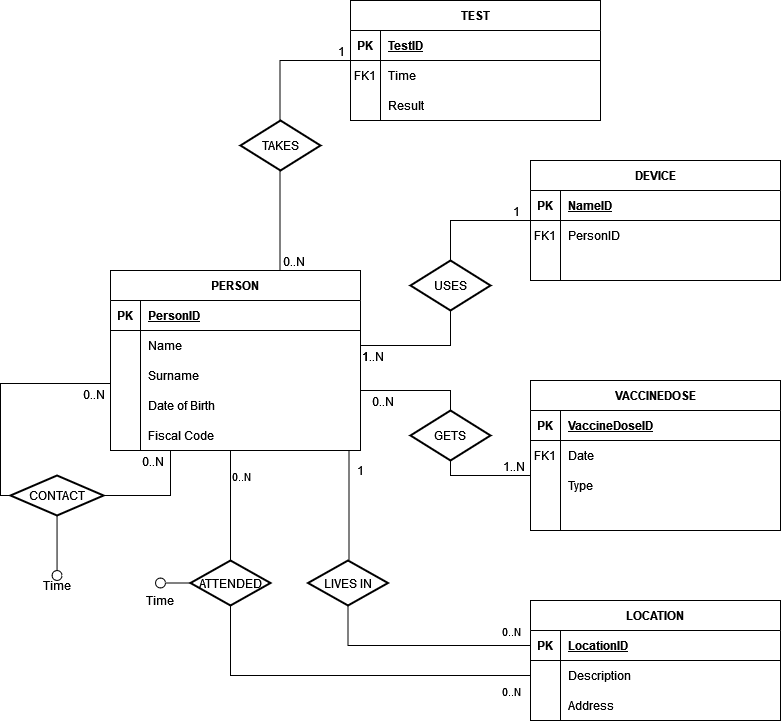
\includegraphics[scale=0.5]{images/e-r.png}
\section{Sample dataset}
A sample dataset has been provided along with this file. In order to import it into your \verb |NEO4J| database, you have to write the following commands.
Since the sample dataset is given in \verb |CSV| files, you can exploit the \verb |LOAD| \verb |CSV| command to load the data (remember to put the files in the \verb |IMPORT| folder) :
\begin{enumerate}
    \item Load the locations: \lstinputlisting[language=SQL]{code/cmd1.txt}
    \item Load the persons: \lstinputlisting[language=SQL]{code/cmd2.txt}
    \item Create the \verb |LIVES| \verb |IN| relationship between users and locations:\lstinputlisting[language=SQL]{code/cmd3.txt}
    \item Create the \verb |ATTENDED| relationship between persons and locations:\lstinputlisting[language=SQL]{code/cmd4.txt}
    \item Load the devices: \lstinputlisting[language=SQL]{code/cmd5.txt}
    \item Create the \verb |OWNS| relationship between persons and devices:\lstinputlisting[language=SQL]{code/cmd6.txt}
    \item Load the tests' dates with the results (remember: a result can be any of \verb |POSITIVE|, \verb |NEGATIVE| or \verb |UNKNOWN|) :\lstinputlisting[language=SQL]{code/cmd7.txt}
    \item Create the \verb |TAKES| relationship between persons and tests:\lstinputlisting[language=SQL]{code/cmd8.txt}
    \item Load the contacts between people: \lstinputlisting[language=SQL]{code/cmd9.txt}
    \item Load the vaccines data about people:\lstinputlisting[language=SQL]{code/cmd10.txt}
    \item Create relationship \verb |GETS| between people and vaccine doses: \lstinputlisting[language=SQL]{code/cmd11.txt}
\end{enumerate}
Now you have a working sample dataset on which you can try the queries of the following paragraph.
\section{Queries and Commands}
The following queries and commands have been developed in order to provide an example of usage of the system for typical usage scenarios.
\subsection{Queries}
We have identified 5 different queries:
\begin{enumerate}
    \item find people with two steps of connection. \\In order to perform this query, we first can consider all the people who live with the considered person (say person 'xxx'):
    \lstinputlisting[language=SQL]{code/query10.txt}
    next, we can consider all the people who our person 'xxx' met in the last 5 days:
    \lstinputlisting[language=SQL]{code/query11.txt}
    then we can consider all the people who our person 'xxx' has been in contact in the last 5 days according to our system:
    \lstinputlisting[language=SQL]{code/query12.txt}
    finally, we take the possible combinations of these three:
    \lstinputlisting[language=SQL]{code/query1end.txt}
    \item find people with the Green Pass (i.e. vaccinated people or people with a negative test made in the last 2 days).\\ First, we have to consider all the people who underwent at least one vaccination (see the assumptions):
    \lstinputlisting[language=SQL]{code/query20.txt}
    next, we consider all the people who made a negative test in the last 2 days:
    \lstinputlisting[language=SQL]{code/query21.txt}
    finally, we compute the union of the 2:
    \lstinputlisting[language=SQL]{code/query22.txt}
    \item find people who violated the isolation.\\ For carrying out this query, the only information we can exploit is the data registered by restaurants, museums, ... According to the assumptions, a person must be at home from the day of a positive test until a negative test, 10 days later:
    \lstinputlisting[language=SQL]{code/query3.txt}
    \item show the number of doses distributed for each brand of vaccine.\\ We have to group all the vaccines and count them:
    \lstinputlisting[language=SQL]{code/query4.txt}
    \item find people who are healed. \\This is the simplest query: we look for all the people with both a positive and a negative test, with the negative test made after the positive one:
    \lstinputlisting[language=SQL]{code/query5.txt}
\end{enumerate}
\subsection{Commands}
We have identified 3 \verb |INSERT| commands to show how the system works:
\begin{itemize}
    \item insert a new person in the system
    \item book a test for a person who was in contact with a positive individual
    \item insert the result of a test
\end{itemize}
\section{Report}
The dataset used has been automatically generated writing some \verb |PHP| scripts and exploiting already existing sample datasets found at \href{https://datasetsearch.research.google.com}{Google Dataset Research}.
\section{User interface}

\end{document}
